% Results, restructured by physical question. Five subsections (JFM structure
% pass): (1) forward closure and conditioning floor; (2) objective/architecture/
% auxiliary-head controls (kept ahead of the mechanism, because architecture and
% wake supervision are confounds); (3) why the rollout works, folding horizon
% dependence into the drift/topology/transport mechanism; (4) where closure
% succeeds and fails in physical space, folding parameter/phase dependence into
% the decoded-field interpretation; (5) wall-pressure observability. The seven
% former run-in \paragraph labels are rewritten as prose. Every result is
% populated.

% Tables for the Results section. Only the two tables discussed at the very top
% of Section 4 (the families overview and the headline closure table) live here
% and are \input at the start of the section. The later tables (conditioning
% floor, latent drift, 2x2 controls) are placed inline next to their first
% reference, further down the section, so floats land near their discussion.

% ---------------------------------------------------------------------------
% TABLE: model families and objectives (new; standard JFM summary table).
% ---------------------------------------------------------------------------
\begin{table}[t]
  \centering
  \caption{Encoder families compared under the matched-predictor protocol of
  \S\ref{sec:methods_protocol}. All three share one autoregressive transformer
  predictor, training recipe, conditioning on $\cvec=(G,D,Y)$, and probe family;
  only the encoder differs. ``Aux.\ heads'' lists the observable supervision
  attached to the encoder. The architecture and auxiliary-head columns differ
  across families, which is why the headline result is attributed to the
  predictive \emph{family} and isolated only by the controls of
  \S\ref{sec:res_controls}.}
  \label{tab:families}
  \small
  \begin{tabular}{l l l l l}
    \toprule
    Family & Objective & Encoder & Latent dim.\ $d$ & Aux.\ heads \\
    \midrule
    JEPA (this work) & predictive (latent) & CNN $+$ ViT & $16,\,32,\,64$ & lift $+$ wake \\
    Reconstructive AE & reconstructive (field) & CNN & $3,\,16,\,32,\,64$ & lift \\
    POD & linear projection & --- & $16,\,32,\,64$ & --- \\
    \bottomrule
  \end{tabular}
\end{table}

% ---------------------------------------------------------------------------
% TABLE: held-out closure (test_b MAE). THIS IS THE HEADLINE TABLE.
% ---------------------------------------------------------------------------
\begin{table}[t]
  \centering
  \caption{Held-out closure across encoder families at $H = 16$ on the $n = 42$
  test\_b encounters, in two modes. \emph{(a)} Representational closure: the mean
  absolute error when each family's per-frame probe is applied to the
  simulation-encoded latent (the latent encoded directly from the held-out field),
  smaller is better. \emph{(b)} Forecast closure: the coefficient of determination
  $R^2$ of the Markov rollout from the impact frame against the simulation
  observable, larger is better (the variance baseline is the held-out split mean,
  so $R^2 < 0$ is worse than predicting that mean). Best per column in bold; the
  forecast panel gives the row mean at right. The wake-enstrophy and circulation
  columns are in native units, the force coefficients dimensionless. This held-out
  forecast $R^2$, not the training-set fit of
  Table~\ref{tab:b1_closure_train_r2}, is the reported closure quality. The
  predictive latent leads in both modes: its representational wake-enstrophy error
  is $2.4$ to $3.0$ times lower than the reconstructive and linear families, and
  its forecast wake-enstrophy $R^2$ is the only one above the predict-the-mean
  floor; the paired per-encounter test is in Table~\ref{tab:paired_closure} and
  full probe values with bootstrap CIs are in Appendix~\ref{app:reg}.}
  \label{tab:closure}
  \small
  \begin{tabular}{l c c c c c c c}
    \multicolumn{8}{c}{\textit{(a) Representational closure: mean absolute error}}\\
    \toprule
    Baseline & $d$ & $C_L$ & $C_D$ & $I_y$ & wake-enst.\ & circ.\ pos.\ & circ.\ neg.\ \\
    \midrule
    JEPA   & 64 & \textbf{0.624} & 0.301 & \textbf{1.901} & \textbf{29.83} & \textbf{0.801} & \textbf{0.715} \\
    JEPA   & 32 & 0.675 & \textbf{0.246} & 2.976 & 37.99 & 1.084 & 1.061 \\
    JEPA   & 16 & 0.627 & 0.267 & 2.883 & 50.09 & 0.939 & 1.322 \\
    \midrule
    Fukami & 3  & 1.074 & 0.384 & 2.327 & 51.70 & 1.110 & 1.886 \\
    Fukami & 32 & 1.038 & 0.368 & 2.195 & 63.94 & 0.946 & 1.789 \\
    Fukami & 64 & 0.989 & 0.340 & 2.421 & 72.90 & 1.057 & 1.904 \\
    Fukami & 16 & 1.133 & 0.421 & 2.424 & 77.26 & 1.158 & 1.837 \\
    \midrule
    POD    & 16 & 1.168 & 0.317 & 2.235 & 89.14 & 1.645 & 1.681 \\
    POD    & 32 & 0.937 & 0.269 & 2.608 & 81.82 & 1.650 & 1.617 \\
    POD    & 64 & 0.872 & 0.291 & 2.245 & 89.31 & 1.660 & 1.800 \\
    \bottomrule
  \end{tabular}

  \vspace{6pt}

  \begin{tabular}{l c c c c c c c c}
    \multicolumn{9}{c}{\textit{(b) Forecast closure: coefficient of determination $R^2$}}\\
    \toprule
    Baseline & $d$ & $C_L$ & $C_D$ & $I_y$ & wake-enst.\ & circ.\ pos.\ & circ.\ neg.\ & mean \\
    \midrule
    JEPA   & 64 & 0.723 & 0.634 & 0.056 & \textbf{0.449} & 0.201 & \textbf{0.607} & \textbf{0.445} \\
    JEPA   & 32 & \textbf{0.751} & \textbf{0.648} & -0.082 & 0.214 & 0.087 & 0.552 & 0.362 \\
    JEPA   & 16 & 0.642 & 0.465 & 0.002 & 0.265 & 0.250 & 0.557 & 0.363 \\
    \midrule
    Fukami & 3  & 0.632 & 0.226 & 0.115 & -0.082 & 0.258 & -0.048 & 0.184 \\
    Fukami & 32 & 0.641 & 0.239 & \textbf{0.205} & 0.007 & \textbf{0.420} & 0.161 & 0.279 \\
    Fukami & 64 & 0.729 & 0.406 & 0.043 & -0.478 & 0.182 & 0.003 & 0.147 \\
    Fukami & 16 & 0.565 & 0.125 & -0.216 & -0.395 & 0.237 & 0.225 & 0.090 \\
    \midrule
    POD    & 16 & 0.499 & 0.364 & -0.515 & -0.129 & -0.230 & 0.340 & 0.055 \\
    POD    & 32 & 0.714 & 0.558 & -0.256 & 0.042 & -0.066 & 0.394 & 0.231 \\
    POD    & 64 & 0.683 & 0.539 & -0.813 & -0.089 & 0.057 & 0.507 & 0.147 \\
    \bottomrule
  \end{tabular}
\end{table}


\subsection{Representational wake closure and the parameter-only floor}
\label{sec:res_closure}

Table~\ref{tab:families} summarises the three encoder families and the protocol.
We distinguish two questions. Does the latent, encoded directly from a held-out
field, render each observable readable by a fixed linear probe (representation
quality, the headline, table~\ref{tab:closure}(a))? And does the predictor, rolled
out from the impact frame, track it (forecast quality, reported as secondary,
table~\ref{tab:closure}(b))? The first isolates the encoder; the second tests the
encoder and the learned dynamics together. The result is established at the
representation level, where the wake is the discriminator, and the rollout is shown
as consistent confirmation rather than the load-bearing test.

The wake is where the families separate. Probed directly from the held-out field
sixteen frames after impact, the predictive latent renders the wake enstrophy
linearly readable at $R^2 = \NumReprWakeJepaTf$ (figure~\ref{fig:fig4_closure}),
while the reconstructive autoencoder and the linear basis are at
$\NumReprWakeFukami$ and $\NumReprWakePod$, both below the predict-the-mean floor.
A nonlinear (kernel-ridge) probe narrows this gap, recovering part of the wake from
the matched-head reconstructive control (\S\ref{sec:res_controls}), so the claim is
that the predictive objective renders the wake \emph{linearly decodable}, not that
the reconstructive encoding discards it irrecoverably. The forces and the
circulations are read off the same latent cleanly, with $C_L$ at
$R^2 = \NumCloReprCLJepaTf$, the negative and positive circulations at
$\NumCloReprCircNegJepaTf$ and $\NumCloReprCircPosJepaTf$, and the drag at
$\NumCloReprCDJepaTf$; the mean over the six observables is
$\NumCloReprMeanSixJepaTf$. The one weak observable is the wall-normal impulse $I_y$
($R^2 = \NumCloReprIyJepaTf$), a mid-plane vorticity diagnostic that even the
energy-optimal linear basis captures only modestly (\S\ref{sec:flow_observables}),
so its weakness is a property of the observable rather than of the predictive
latent. The same ordering holds on the training, validation, and extrapolation
(test\_c) splits reported below.

\begin{figure}
  \centering
  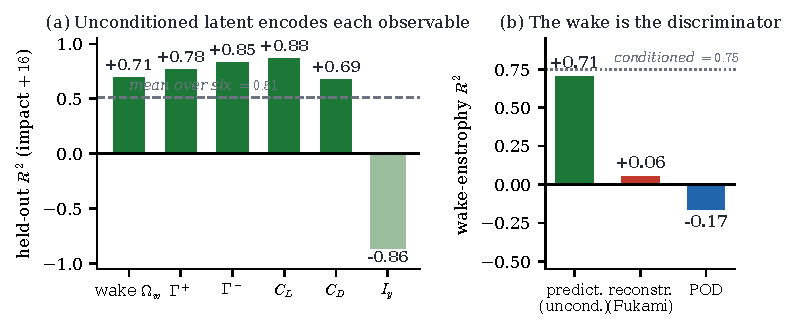
\includegraphics[width=\linewidth]{sections/figures/results/fig4_closure.pdf}
  \caption{Representational closure of the predictive latent at $H = 16$ after gust
  impact, the headline result. (a) Held-out $R^2$ of a fixed linear probe applied to
  the simulation-encoded latent (no rollout) for each of the six observables, on the
  in-distribution test set (test\_b, $n = 42$); the dashed line marks the mean over
  the six and the one weak observable, the mid-plane impulse $I_y$, is shaded light.
  (b) The wake-enstrophy $R^2$ across families: the predictive latent
  ($\NumReprWakeJepaTf$) against the reconstructive autoencoder
  ($\NumReprWakeFukami$) and the linear basis ($\NumReprWakePod$), each at $d = 64$.
  The wake is the discriminator, and only the predictive latent renders it linearly
  readable.}
  \label{fig:fig4_closure}
\end{figure}

The rollout points the same way and is read as confirmatory, not as the headline
(table~\ref{tab:closure}(b) and figure~\ref{fig:traces}). A matched transformer
predictor is trained on each family's latents under one protocol, and rolled out
from the full pre-impact context; probing the wake enstrophy at $H = 16$, the
forecast $R^2$ is $\NumCloFcstWakeJepaTf$ for the predictive latent, ahead of
$\NumCloFcstWakeFukami$ for the reconstructive autoencoder and
$\NumCloFcstWakePod$ for the linear basis. The forecast ordering is the same as the
representational one but compressed, which is why we lead with the representation:
the families separate most cleanly at the encoder, and the rollout confirms rather
than carries the result. The forecast advantage is not statistically separable
under case-level clustering (\S\ref{sec:res_drift} and
table~\ref{tab:paired_closure}), so we present it as consistent tracking, not as a
forecast claim. On the extrapolation set (test\_c, $G = +4$) the predictive
wake-enstrophy forecast stays the strongest of the three while the integrated
forces collapse, consistent with the three-dimensional observability boundary of
\S\ref{sec:flow_physics}.

\begin{figure}
  \centering
  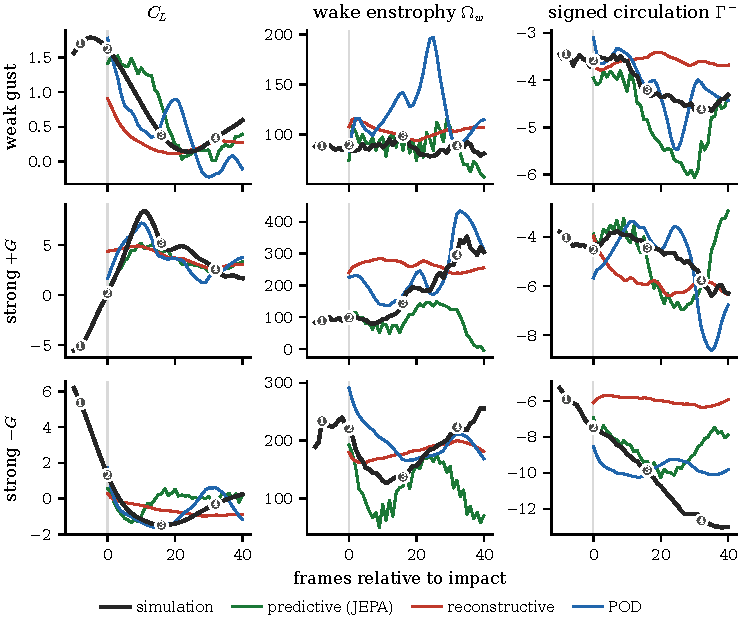
\includegraphics[width=\linewidth]{sections/figures/results/figA_traces.pdf}
  \caption{The predictive rollout tracks the encounter, shown qualitatively.
  Predicted observables through representative held-out encounters (rows), for the
  lift coefficient, the wake enstrophy, and the negative circulation (columns). The
  simulation is the bold reference; the rollout of the predictor, started from the
  pre-impact context, is the coloured line, and the dashed line is the
  reconstruction from the encoded latent. The rollout tracks the
  wake observables through the leading-edge-vortex peak and into recovery before
  drifting gently at long times. We report this as qualitative tracking, not as a
  closure $R^2$. Numbered glyphs mark the four encounter stages used throughout:
  baseline, impact, peak load, and recovery.}
  \label{fig:traces}
\end{figure}

The representational wake separation is the statistically robust core of the
result. A per-encounter paired test (table~\ref{tab:paired_closure}), which cancels
the encounter-to-encounter difficulty of the held-out set that every model shares,
shows the predictive latent carrying the smaller wake-enstrophy error under direct
encoding by a paired margin of $\NumPairedWakeRepr$ (case-clustered $95\%$ CI
$[\NumPairedWakeReprlo, \NumPairedWakeReprhi]$, excluding zero). We report the
multiplicity correction at two levels and state honestly where the advantage
stops: the representational wake-enstrophy advantage survives the pre-registered
encounter-level family correction (one of $\NumHolmSurvivors$ of twelve paired
tests that survive Holm, together with the lift and the negative circulation),
but it does not survive the stricter case-level correction, where the smaller
number of held-out cases widens the interval. The forecast advantage points the
same way but survives neither. All six observables are reported in both modes, not
a selected subset, and the ordering is not uniform: the predictive latent leads on
the spatially distributed wake observables (enstrophy and negative circulation),
which is precisely the paper's claim. This separation is confirmed by the
mechanistic evidence of \S\ref{sec:res_drift} (the drift departure spectrum and the
no-gust limit-cycle topology), where the predictive and reconstructive families
separate consistently.

\begin{table}
  \centering
  \caption{Parametric (model-free) floor at $H = 16$ after impact. A
  cross-validated ridge regressor maps the gust parameters $\cvec = (G,D,Y)$
  directly to each observable, with no latent input, fit on the training cases and
  read out on the in-distribution test split under the closure protocol
  ($R^2 = 1 - \mathrm{SSE}/\mathrm{SST}$ about the held-out mean). This is the
  model-free baseline: the predictive latent beating it (last column, the
  representational closure of table~\ref{tab:closure}(a)) shows the representation
  carries flow state the parameters alone do not supply. On wake enstrophy the
  floor is negative ($R^2 = \NumFloorWake$): the gust parameters alone do worse than
  the held-out mean sixteen frames after impact, because the wake is then governed
  by the unfolding dynamics rather than by the release condition, whereas the
  predictive latent reads it at $\NumReprWakeJepaTf$. On the forces, which track the
  gust forcing more directly, the floor is high.
  }
  \label{tab:parametric_floor}
  \small
  \fittab{\begin{tabular}{l c c}
    \toprule
    Observable & parametric floor (test\_b $R^2$) & predictive repr.\ (test\_b $R^2$) \\
    \midrule
    $C_L$          & \NumFloorCL      & \NumCloReprCLJepaTf \\
    $C_D$          & \NumFloorCD      & \NumCloReprCDJepaTf \\
    $I_y$          & \NumFloorIy      & \NumCloReprIyJepaTf \\
    wake-enstrophy & \NumFloorWake    & \NumReprWakeJepaTf \\
    circ.\ pos.\   & \NumFloorCircPos & \NumCloReprCircPosJepaTf \\
    circ.\ neg.\   & \NumFloorCircNeg & \NumCloReprCircNegJepaTf \\
    \bottomrule
  \end{tabular}}
\end{table}

The parametric floor (table~\ref{tab:parametric_floor}) confirms that the wake
closure is not something the gust parameters supply on their own. Mapping
$\cvec = (G,D,Y)$ to each observable at $H = 16$ with cross-validated regressors,
the floor on wake enstrophy is negative ($R^2 = \NumFloorWake$ for the linear
regressor, $\NumParamFloorWakeKrr$ for the nonlinear one): the parameters alone do
worse than predicting the held-out mean, while the predictive latent reads the wake
at $\NumReprWakeJepaTf$, clearing the floor by roughly $0.9$. The floor is by
construction strong on the observables that track the gust forcing directly, the
lift ($\NumFloorCL$) and the negative circulation ($\NumFloorCircNeg$): the
predictive advantage is specific to the spatially distributed wake, not uniform
across observables, and this is the paper's central distinction between the
integrated forces, which the release condition largely fixes, and the wake, which
it does not. The wake claim therefore rests on the representational closure
(table~\ref{tab:closure}(a)), the per-encounter paired test
(table~\ref{tab:paired_closure}), and the drift mechanism (\S\ref{sec:res_drift}),
with the parametric floor establishing that the gust parameters do not supply the
wake state the latent encodes.

\subsection{Objective, architecture, and auxiliary-head controls}
\label{sec:res_controls}

The representational result of \S\ref{sec:res_closure} is established, but the
predictive latent \emph{family} as configured renders the wake readable for reasons
we have not yet separated: the predictive encoder differs from the reconstructive
baseline not only in its training objective but also in its CNN$+$ViT architecture
and its $80$-dimensional wake supervision. Because the architecture and the wake
supervision are confounds, we isolate the cause here, before turning to why the
rollout stays on the manifold (\S\ref{sec:res_drift}). The controls in
table~\ref{tab:controls_2x2} are the decisive crossing, run directly on the same
models the paper reports and scored at the representational endpoint: a
$2 \times 2$ crossing of objective \{predictive, reconstructive\} with architecture
\{CNN, CNN$+$ViT\} at matched $d = 64$, with the auxiliary heads matched across all
four cells, together with a predictive variant from which the wake head is removed.
The decisive question is whether the predictive objective renders the wake readable
more than the reconstructive one once the architecture and the wake supervision are
held in common.

\begin{table}
  \centering
  \caption{Objective $\times$ architecture controls (decisive experiment), scored
  at the representational endpoint on the in-distribution test split. Held-out
  representational wake-enstrophy $R^2$ at $H = 16$ (test\_b, fixed linear probe on
  the simulation-encoded latent, seed mean) for the four cells crossing
  \{predictive, reconstructive\} with \{CNN, CNN$+$ViT\} at $d = 64$, with the
  auxiliary heads (the instantaneous lift plus the $80$-dimensional wake head)
  matched across all four cells, plus a predictive variant with the wake head
  removed. Predictive renders the wake readable at both architectures, while both
  reconstructive cells stay low; removing the wake head from the predictive model
  collapses wake readability to the floor, so the wake supervision is also
  necessary. The CNN and CNN$+$ViT predictive columns do not separate, so the ViT
  is not the driver.}
  \label{tab:controls_2x2}
  \small
  \fittab{\begin{tabular}{l l l c}
    \toprule
    Objective & Encoder & Aux.\ heads & repr.\ wake-enst.\ $R^2$ \\
    \midrule
    predictive     & CNN$+$ViT & lift $+$ wake & $\mathbf{\NumReprWakeJepaTf}$ \\
    predictive     & CNN       & lift $+$ wake & $\NumReprWakeCtrlPredCnn$ \\
    reconstructive & CNN$+$ViT & lift $+$ wake & $\NumReprWakeCtrlReconCnnVit$ \\
    reconstructive & CNN       & lift $+$ wake & $\NumReprWakeCtrlReconCnn$ \\
    \midrule
    predictive     & CNN$+$ViT & lift only     & $\NumReprWakeCtrlPredVitNowake$ \\
    \bottomrule
  \end{tabular}}
\end{table}

The controls (table~\ref{tab:controls_2x2}) give a two-part answer, and we state
both. First, the predictive objective renders the wake readable at \emph{both}
architectures with the auxiliary heads matched: the representational
wake-enstrophy $R^2$ is $\NumReprWakeJepaTf$ for the predictive CNN$+$ViT and
$\NumReprWakeCtrlPredCnn$ for the predictive CNN, while both reconstructive cells
stay low ($\NumReprWakeCtrlReconCnnVit$ at CNN$+$ViT, $\NumReprWakeCtrlReconCnn$ at
CNN). The objective, not the architecture, carries the advantage: the two
predictive columns do not separate, so the ViT is not the driver. Second, and
equally important, the wake-observable supervision is necessary: the predictive
model with the wake head removed collapses to a representational wake $R^2$ of
$\NumReprWakeCtrlPredVitNowake$, at the floor and below every other predictive
cell. The result therefore requires the predictive objective \emph{and} the wake
supervision together; it is not a property of the objective in isolation, nor of
the architecture, nor of the wake head attached to an arbitrary objective (the
reconstructive cells carry the same wake head and do not reach the predictive
readability). We claim, accordingly, that the predictive objective renders the
wake linearly readable over the reconstructive objective at matched architecture
and matched supervision, with the auxiliary wake head a necessary component of the
configuration that achieves it.

The latent dimension is the remaining control. The representational wake closure
holds on a plateau from $d = 64$ down to $d = 16$ ($R^2 = \NumCloReprWakeJepaTfDSixtyfour$,
$\NumCloReprWakeJepaTfDThirtytwo$, and $\NumCloReprWakeJepaTfDSixteen$ at $d = 64$, $32$,
and $16$) and falls off below, so the reported $d = 64$ sits on the plateau and the
wake is not recoverable at the smallest dimensions on this dataset. The latent code
is correspondingly distributed rather than concentrated in a few coordinates, which
\S\ref{sec:res_code} makes quantitative.

\subsection{Why the latent stays on the manifold: drift, topology, and transport}
\label{sec:res_horizon}
\label{sec:res_drift}

The controls attribute the wake advantage to the predictive objective trained
with wake supervision, and the representation is where that advantage is
established. A separate question is whether the latent is usable under rollout,
since a planner queries a forward model at the states its own rollout reaches. The
answer is geometric: the unconditioned predictive latent stays on its encoded
manifold while the reconstructive one drifts off, which we establish first as a
horizon-resolved rollout drift and then with three coordinate-free diagnostics of
the rollout itself.

The unconditioned rollout drifts gracefully. Rolling the unconditioned predictor
forward and measuring the relative deviation of the rolled latent from the latent
encoded directly from the simulation, as a fraction of the encoded-latent scale, the
drift grows gradually with horizon and stays bounded
(figure~\ref{fig:drift_uncond}), and it tracks the conditioned model closely, so
removing the gust parameters does not destabilise the rollout. This is the property a
forward model needs and it is why the qualitative rollout of figure~\ref{fig:traces}
tracks the encounter through impact before drifting only at long times. We do not
attach a forecast $R^2$-versus-horizon headline to this rollout; the representational
closure of \S\ref{sec:res_closure} carries the result, and the rollout is shown to be
on-manifold and usable.

\begin{figure}
  \centering
  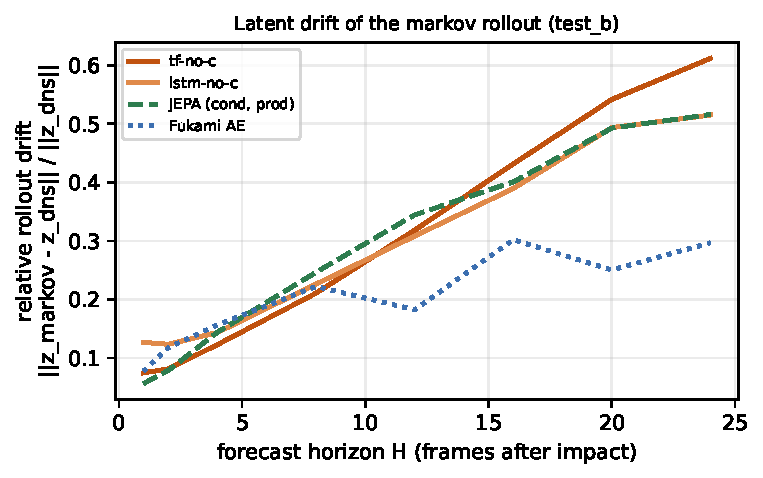
\includegraphics[width=0.7\linewidth]{sections/figures/results/fig_horizon_sweep.pdf}
  \caption{Relative drift of the unconditioned rollout on test\_b versus forecast
  horizon $H$, measured as the deviation of the rolled latent from the
  simulation-encoded latent normalised by the encoded-latent scale,
  $\lVert \widehat{\zvec}_{\text{rollout}} - \zvec_{\text{DNS}}\rVert /
  \lVert \zvec_{\text{DNS}}\rVert$. The unconditioned transformer predictor (tf-no-c)
  and a recurrent unconditioned variant (lstm-no-c) drift gradually and track the
  conditioned production model closely, so dropping the gust parameters does not
  destabilise the rollout. This is a deviation diagnostic of the unconditioned model,
  not a forecast-$R^2$ headline; the family-separating drift is the Mahalanobis
  manifold-departure of table~\ref{tab:latent_drift}.}
  \label{fig:drift_uncond}
\end{figure}

The drift behaviour points to a geometric cause, which the rest of this
subsection establishes three ways that do not
depend on the latent coordinates: a distance that shows whether the rollout leaves
the training manifold, a topology that shows whether the encounter stays a single
cycle, and an optimal-transport metric that shows whether latent distance tracks the
physical rearrangement of the flow. Together they test the one property a predictive
objective confers and a reconstruction objective does not, that the latent metric
stays aligned with the transport geometry under the predictor step, so the rollout
remains close to the encoded manifold.

\begin{table}
  \centering
  \caption{Latent-drift diagnostic on test\_b at $H = 16$. The Mahalanobis
  distance of the rolled-out latent is reported alongside that of the
  simulation-encoded latent in the same reference distribution; their ratio
  $r = d_{\text{Mahal, Markov}} / d_{\text{Mahal, DNS}}$ measures how far the
  autoregressive rollout has left the training manifold. A ratio near one means
  the rollout stays in distribution. The unconditioned predictor used throughout
  the paper drifts comparably to the values shown: its relative rollout drift grows
  gracefully and stays bounded, tracking the conditioned model closely, so removing
  the gust parameters does not destabilise the rollout.}
  \label{tab:latent_drift}
  \small
  \fittab{\begin{tabular}{l c c c c}
    \toprule
    Baseline & $d$ & $d_{\text{Mahal, ref}}$ & $d_{\text{Mahal, rollout}}$ & ratio $r$ \\
    \midrule
    Fukami & 64 & 2.92 & 28.96 & \textbf{9.90} \\
    JEPA   & 64 & 8.08 & 6.84  & 0.85 \\
    JEPA   & 32 & 5.43 & 4.65  & 0.86 \\
    POD    & 64 & 7.74 & 6.27  & 0.81 \\
    \bottomrule
  \end{tabular}}
\end{table}

First, the latent-drift diagnostic (table~\ref{tab:latent_drift})
measures how far each rollout leaves its training manifold. After $H = 16$ steps
the reconstructive rollout sits an order of magnitude further from its training
distribution than its simulation-encoded counterpart (ratio $9.90$), while the
predictive and linear rollouts remain within it (ratios $0.85$ and $0.81$). This
is the mechanism behind the closure gap: the probe attached to a drifted rollout
is queried outside the support it was fit on, so its output degrades for reasons
unrelated to the predictor's one-step quality. A reconstruction objective places
latent codes wherever the decoder finds convenient and does not constrain the
geometry to be predictable in time; the predictive objective, regularised
against collapse, produces a latent that supports stable rollout by
construction. The pre-impact inference of the impact lift makes the same point
from the encoder side: an oracle probe on the simulation-encoded predictive
latent recovers the impact $C_L$ at $R^2 = 0.683$ at every lead time, whereas
the same oracle on the reconstructive latent is negative ($-0.185$), a
representation failure rather than a probe failure, since no probe can recover
information the latent does not carry. The reconstructive rollout therefore fails
because the latent has left the manifold the probe was fit on, not because the
predictor step is inaccurate.

Distance alone understates the geometric content of the
result, so we next examine the trajectory topology. A gust encounter departs the baseline limit cycle, executes the
LEV-formation and shedding excursion, and relaxes back toward it without closing
within the window (\S\ref{sec:res_param_phase}); in the encoded latent the
excursion nonetheless has the topology of a single cycle \citep{smith2024}. We characterise this with persistent homology, which
identifies the persistent one-dimensional cycle ($H_1$ generator) of a
trajectory by a Vietoris--Rips filtration \citep{smith2024}, applied here to four
latent point clouds per encounter: the simulation-encoded predictive latent, its
rollout, the simulation-encoded reconstructive latent, and its rollout
(figure~\ref{fig:persistence}). The coordinate-free signature is not the survival
of a single generator's lifetime, which is confounded by scale (the
reconstructive rollout drifts into a large diffuse cloud that still supports a
long-lived but non-canonical loop, so the rollout-to-encoded lifetime ratio is
near one for both families and does not separate them). It is the
\emph{generator count} of the simulation-encoded latent itself: the unconditioned
predictive encoding produces a clean single cycle (median one significant $H_1$
generator on test\_b, $52\%$ of encounters with exactly one), while the
reconstructive encoding fragments into several (median $3.5$, $71\%$ with three or
more; Mann--Whitney $p = 4.9 \times 10^{-9}$). The predictive latent has the clean limit-cycle topology of the
physical encounter; the reconstructive latent does not. This is consistent with
the curvature geometry of \S\ref{sec:res_param_phase}: the impact frame is a
curvature minimum of the predictive trajectory, a smooth pass-through rather than
a sharp corner, so the cycle it traces is a single well-formed loop. The result
at $d = 32$ is the same (single predictive loop versus reconstructive
fragmentation). The separation is robust to the two free choices of the analysis,
following the convergence protocol of \citet{smith2024}: across noise floors from
$2\%$ to $15\%$ of the cloud diameter and trajectory subsampling down to $60$
points the predictive median stays at one generator and the Mann--Whitney
separation holds at $p < 10^{-3}$, and it survives case-level clustering ($10$ of
$10$ cases, signed-rank $p = 10^{-3}$ at the canonical setting). At the most
aggressive $20\%$ floor, or under heavy subsampling to $30$ points, the spurious
reconstructive generators are themselves filtered and the two medians converge, so
the exact $p$ is floor- and sampling-dependent while the median-count separation
is not (Appendix~\ref{app:reg}).
\begin{figure}
  \centering
  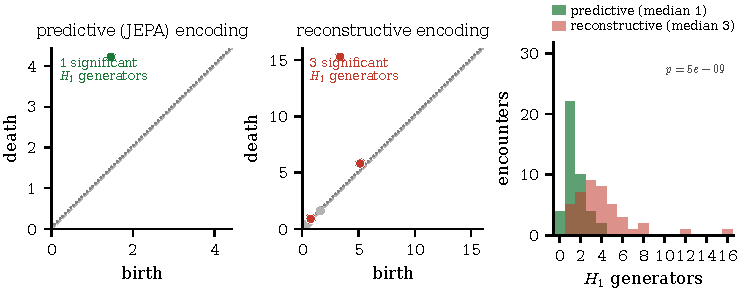
\includegraphics[width=0.98\linewidth]{sections/figures/results/fig_persistence.pdf}
  \caption{Persistent homology of the latent encounter on test\_b. Left and
  centre: representative Vietoris--Rips $H_1$ persistence diagrams of the
  simulation-encoded predictive and reconstructive latents; coloured points are
  significant generators (lifetime above the dotted noise floor) and grey points
  are noise. Right: the distribution of the significant-$H_1$ generator count over
  the $42$ held-out encounters, the scale-free signal. The unconditioned predictive
  encoding is a single clean loop (median one generator) while the reconstructive
  encoding fragments (median three to four; Mann--Whitney one-sided
  $p = 4.9\times10^{-9}$).}
  \label{fig:persistence}
\end{figure}

The third test makes the geometry physical by comparing latent distances with the
unbalanced optimal-transport distance between vorticity fields. Euclidean distance
between vorticity
fields is insensitive to the spatial transport of structures, whereas an
unbalanced optimal-transport (OT) distance measures the cost of rearranging one
field into another and so tracks advection of the LEV and shear layer
\citep{tran2026}. Computing the OT distance between simulation fields along an
encounter gives a physical transport geometry against which the latent metric
can be checked: the prediction is that distances in the predictive latent track
the OT distances more faithfully than distances in the reconstructive latent, so
that iterating the predictor step keeps the rollout closer to the data manifold.
The
prediction holds: the per-encounter Spearman correlation between the latent
distance matrix and the simulation OT-distance matrix on test\_b is $0.61$ for
the predictive latent against $0.45$ for the reconstructive latent, a margin of
$0.16$. The predictive latent metric is therefore more aligned with the physical
transport geometry, in this empirical distance-matrix sense, consistent with a
rollout that remains closer to the encoded manifold. We report this per encounter
rather than pooled across encounters, and we are explicit that the statistic is
trajectory-local: pooling across encounters conflates the within-encounter geometry
with a between-encounter latent-norm scale that the drift-prone reconstructive
latent inflates, which reverses the pooled statistic ($0.41$ predictive against
$0.63$ reconstructive) and is itself a symptom of the same drift. We therefore claim
trajectory-local transport consistency, not a global isometry.

\subsection{Where the wake is kept and where it is lost in physical space}
\label{sec:res_param_phase}
\label{sec:res_physical}

The mechanism explains why the predictive rollout stays on the manifold; we now
ask where in the gust envelope, and where in the flow field, the latent keeps the
wake. The parameter dependence reveals one clear weakness, and it is worth noting
that the latent encodes these parameters despite never being trained on them.
Probing the predictive latent for the gust parameters on test\_b recovers the gust
strength $G$ and the core diameter $D$ ($R^2 = 0.46$ and $0.80$) but barely resolves
the wall-normal offset $Y$ ($R^2 = 0.10$). This is a property of the data rather than of the
architecture: the training mass concentrates near $Y \approx 0$, so encounters
at different offsets within the envelope are weakly separated along $Y$, and the
latent inherits that weakness. Any deployment-time parameter estimate should
treat $Y$ as a nuisance variable the encoder resolves only weakly.

The same latent can also be read relative to the undisturbed shedding cycle.
Because the undisturbed wake
is a limit cycle (\S\ref{sec:flow_physics}), an encounter is naturally described
by its phase and amplitude relative to that cycle, the same reduction used to
design gust-mitigation control for these flows \citep{fukami2024control}. Reading
the predictive latent this way makes ``recovery'' precise: it is the return of
the latent trajectory to the baseline limit cycle. The predictive latent of the
undisturbed case does trace a closed periodic orbit
(figure~\ref{fig:phase_amplitude}): concatenating the four no-gust episodes, the
return distance is $1.0\%$ of the orbit diameter, and the four episodes overlap
the same loop, with a shedding period of about $56$ frames ($2.8$ convective
times, Strouhal number near $0.36$). A phase advances monotonically along it
(via the Hilbert analytic signal of the two leading latent principal components),
though the orbit lives in more than two dimensions, so the phase is a reduction
rather than a complete coordinate. A gust encounter departs this orbit and is
carried back toward it under the predictive rollout while the reconstructive
rollout departs further: the median return-to-orbit distance on test\_b is
smaller for the predictive latent at every horizon, and the separation is
bootstrap-robust at $H = 64$ (predictive $8.70$ versus reconstructive $9.96$,
$95\%$ confidence interval on the paired difference $[1.13, 3.25]$), marginal at
$H = 32$. One caveat applies: the simulation gust
trajectories do not themselves fully return to the baseline orbit within the
$120$-frame window. That window is the gust-release period itself
($6\,t/c$ at $\Delta t = 0.05\,t/c$, with impact near $2\,t/c$), so only about
$4\,t/c$ of post-impact relaxation is ever observed before the next gust is
released, short of a full return; this is a window-length limitation set by the
gust-release cadence, and at fixed core diameter it is not strength-dependent.
The comparison therefore measures the relative drift direction (the predictive
rollout contracts toward the orbit, the reconstructive one expands away), not a
completed physical recovery. The result is the same at $d = 32$.
This limit cycle and the persistent cycle of the previous subsection are the same
object viewed dynamically and topologically.
\begin{figure}
  \centering
  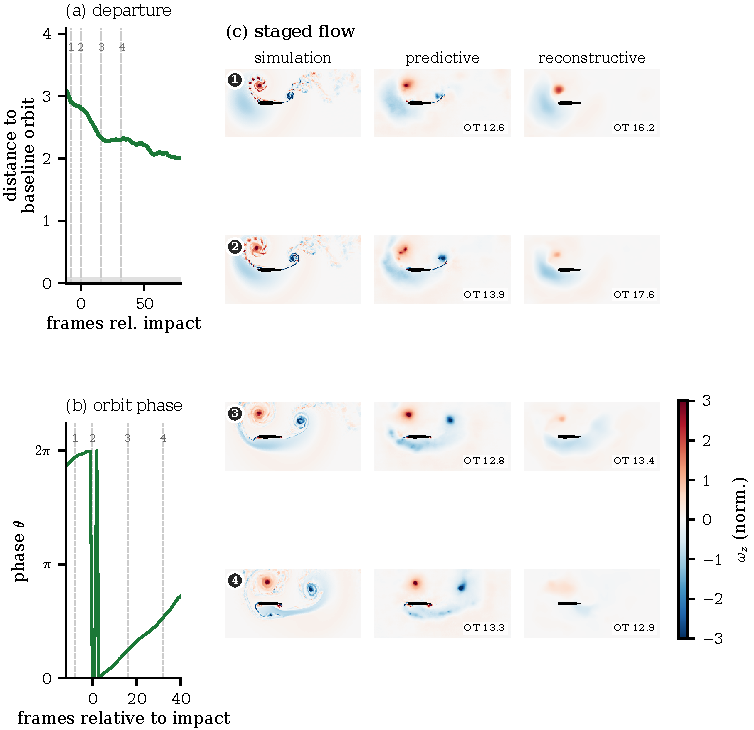
\includegraphics[width=\linewidth]{sections/figures/results/figC_cycle.pdf}
  \caption{The gust encounter in the predictive latent, for a strong negative
  gust $(G, D, Y) = (-3.0, 1.5, -0.1)$. (a) Distance of the gust trajectory to the
  baseline orbit (full latent, in units of the orbit diameter; the grey band is
  the baseline orbit thickness): the encounter departs the baseline cycle and only
  partially relaxes back, without closing within the inter-gust window;
  the single-cycle topology of the encoded latent
  is established coordinate-free in figure~\ref{fig:persistence}. (b) The orbit
  phase relative to the impact frame. (c) Mid-plane vorticity at the four stages
  (rows) for the simulation, the predictive decode, and the reconstructive decode
  (columns); the predictive decode localises the impingement while the
  reconstructive decode collapses, with the optimal-transport field distance
  between each decode and the simulation annotated at each stage (largest for the
  reconstructive decode near impact). The numbered stages are those of
  figure~\ref{fig:traces}.}
  \label{fig:phase_amplitude}
\end{figure}

We can also locate where in the envelope the predictive advantage concentrates.
Rather than a
per-stratum closure table, which the present test set is too small to populate,
we read the per-encounter paired improvement
$\Delta e = e_{\text{AE}} - e_{\text{JEPA}}$ in held-out wake-enstrophy error
directly against each gust axis with a locally weighted regression and a
bootstrapped band (figure~\ref{fig:error_maps}). The advantage is not uniform
across the envelope. It grows with the gust core diameter $D$ (Spearman
$\rho = 0.42$ on the encoded latent, $0.53$ under forecast) and toward
off-midplane wall-normal offset $Y$ ($\rho = 0.49$ and $0.45$), both significant,
while its dependence on the gust strength $G$ is weak on the encoded latent and
moderate under forecast. The predictive advantage therefore concentrates away
from the $Y \approx 0$ training mass and at the larger cores that most reorganise
the wake, consistent with the weak $Y$ resolution of the probe above. The
shedding phase at impact, the axis the gust-response literature emphasises
\citep{fukami2024control}, is only weakly sampled by this dataset: impact is fixed
near a single convective instant while the gust recurs about every two shedding
periods, so the encounters fall into essentially two phase clusters and a
phase-resolved trend is not identifiable here, which a design that varies the
impact phase would isolate.
\begin{figure}
  \centering
  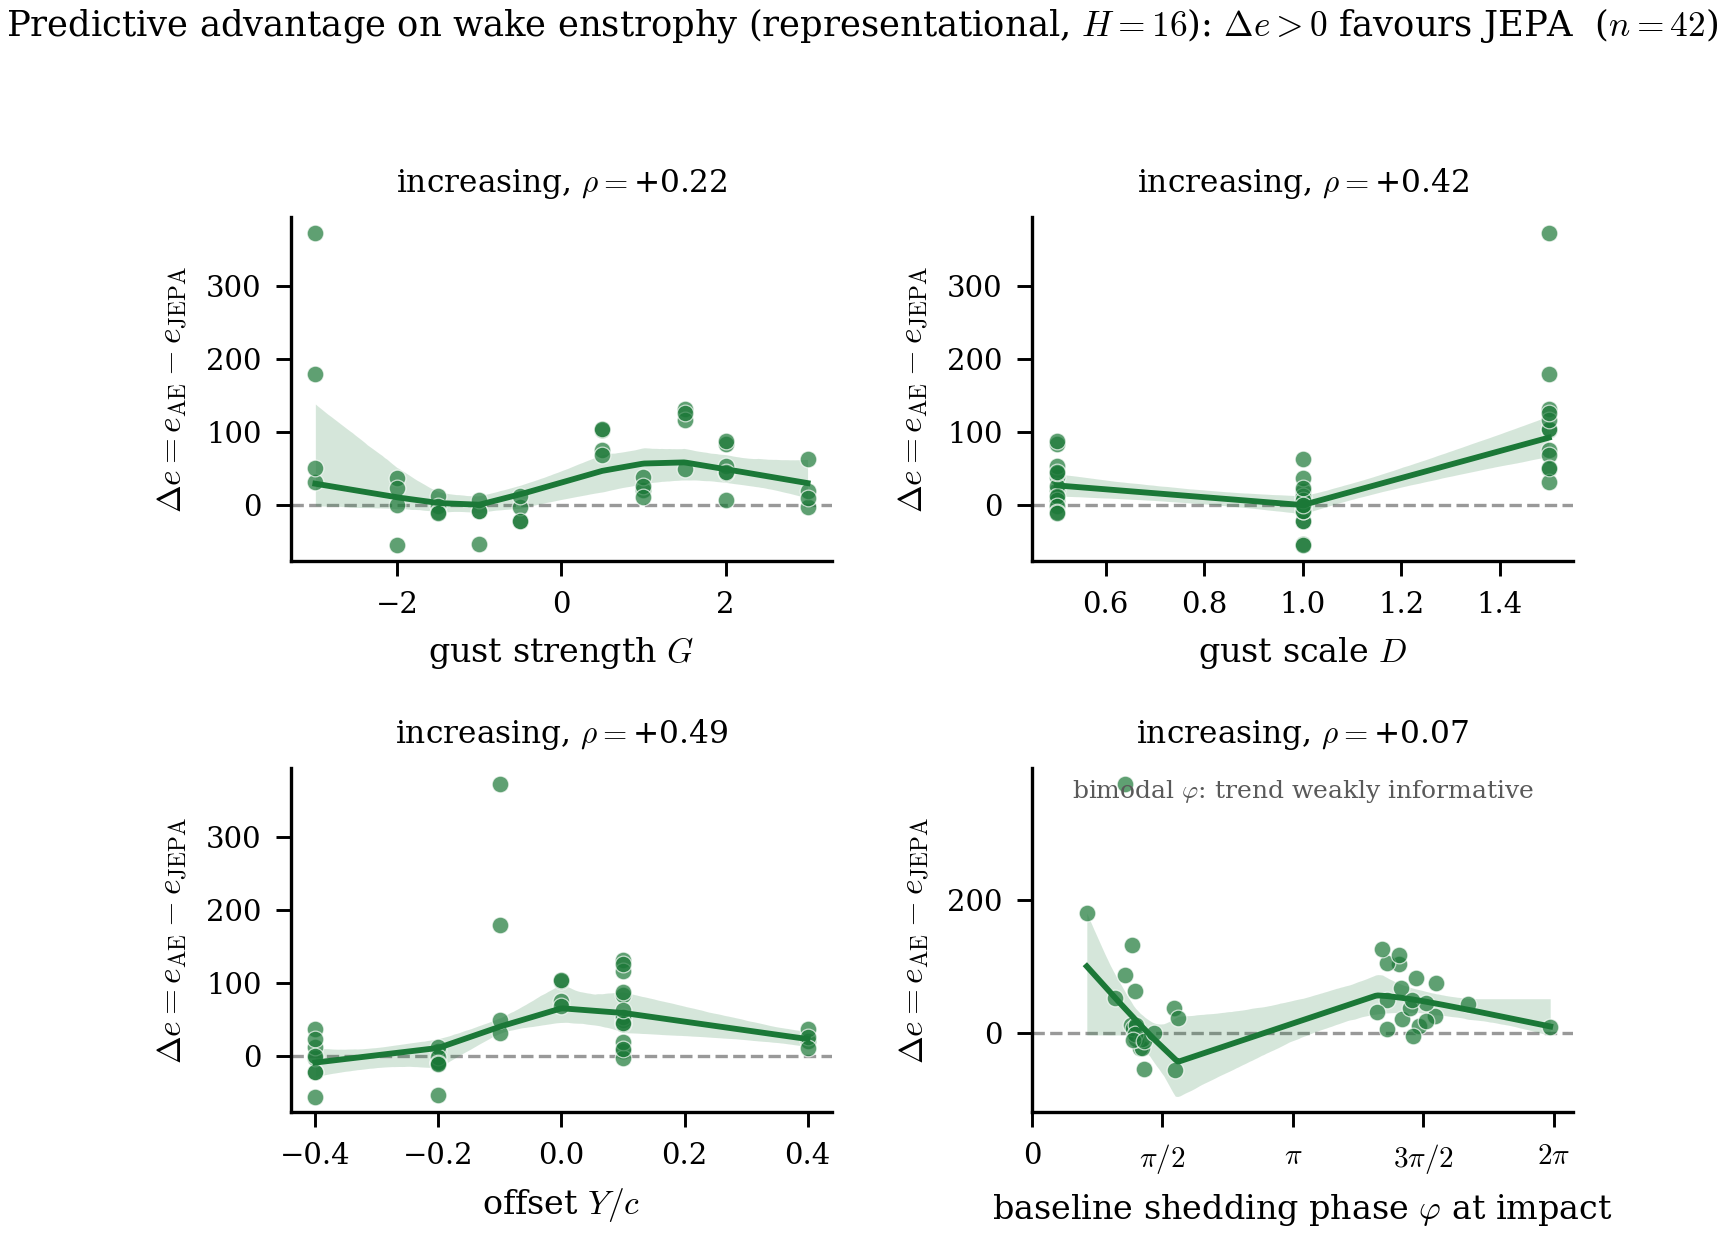
\includegraphics[width=\linewidth]{sections/figures/results/fig_error_maps.png}
  \caption{Per-encounter paired improvement
  $\Delta e = e_{\text{AE}} - e_{\text{JEPA}}$ in held-out wake-enstrophy error
  against the gust strength $G$, core diameter $D$, wall-normal offset $Y$, and
  the baseline shedding phase at impact $\phi$ (test\_b, $n = 42$); positive
  $\Delta e$ means the predictive latent carries the smaller error. Each panel
  shows the per-encounter values, a locally weighted (LOWESS) trend, and a
  bootstrap band over encounters. The predictive advantage grows with $D$ and
  toward off-midplane $Y$; the shedding-phase axis falls into two clusters because
  impact is fixed near a single convective instant.}
  \label{fig:error_maps}
\end{figure}

These parameter and phase readings are statements about numbers; the encounter is
itself a statement about
vortices. Decoded and reconstructed vorticity fields on held-out encounters
(figure~\ref{fig:recon}) connect the two, with one
methodological caution and one new metric. Two scoping points apply throughout
this subsection. The fields are encode-decode reconstructions, the visualisation
decoder applied to the simulation-encoded latent, so the quantitative comparisons
report the decoder's ceiling on what each latent carries from a faithfully encoded
field, not a forecast rollout, whose latent leaves the data manifold for the
reconstructive baseline (\S\ref{sec:res_drift}). And every quantitative
physical-space claim is made on the validated large-scale band ($\sigma/c = 0.05$);
the visualisation decoder is blurry at small scale by construction, so the
large-scale leading-edge vortex and shear layer are tracked meaningfully while
full-resolution and small-scale field fidelity are not claimed.

\begin{figure}
  \centering
  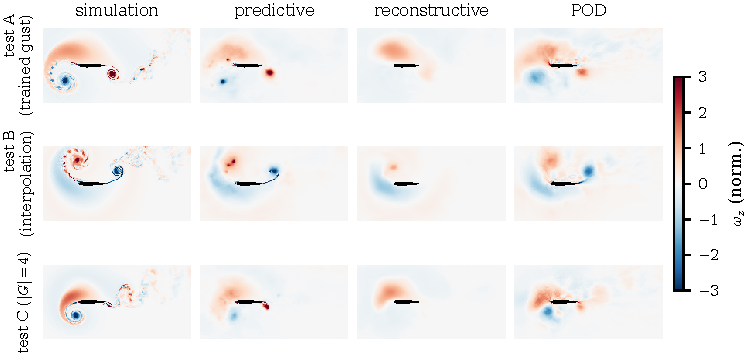
\includegraphics[width=\linewidth]{sections/figures/results/figD_reconstructions.pdf}
  \caption{Decoded vorticity at the impact frame on held-out encounters from the
  three splits (rows: a trained-gust test\_a encounter, an interpolation test\_b
  encounter, and a $|G| = 4$ test\_c encounter) for the simulation and the
  predictive, reconstructive, and POD decodes (columns). The predictive decoder is
  blurry by design but localises the impingement; the reconstructive autoencoder
  collapses toward a near-uniform field on the held-out interpolation condition,
  while the linear basis is amplitude-accurate. All families degrade in the
  $|G| = 4$ regime, reported as the observability boundary of
  \S\ref{sec:flow_physics} rather than as a generalisation claim. Field-space
  similarity is reframed by the optimal-transport metric introduced below.}
  \label{fig:recon}
\end{figure}

The caution is that field-space similarity scores are misleading here. On a
held-out interpolation encounter the reconstructive autoencoder attains a high
structural similarity yet a peak reconstructed vorticity magnitude of only
$0.36$ against a target peak near $9.7$: it has collapsed to a near-uniform mean
field and lost the vortex-impingement signature, and the high similarity merely
reflects bulk agreement with a field that is itself mostly quiescent away from
the impact region. The predictive latent localises the impingement at the right
position and sign (peak magnitude $5.31$) but its visualisation decoder is blurry
by construction, and the linear basis is amplitude-accurate (peak $4.10$) since
its objective is amplitude-optimal.

The new metric resolves the caution. An unbalanced optimal-transport distance
between the reconstructed and the simulation fields, computed for the positive
and negative vorticity separately and summed \citep{tran2026}
(entropic unbalanced Sinkhorn transport cost with a KL marginal relaxation, fields pooled to $48 \times 24$ for tractability),
penalises the collapsed reconstruction correctly and reorders the comparison
where structural similarity misleads (figure~\ref{fig:ot}). At the impact frame
on test\_b the transport distance is largest for the reconstructive autoencoder
($11.25$) and smaller and comparable for the predictive decode ($9.90$) and the
linear basis ($9.95$). The instructive case is the linear basis: it carries the
\emph{highest} structural similarity of the three ($0.69$ against $0.65$ for the
predictive decode), which would wrongly crown the energy-optimal reconstruction
as the best, yet under transport it is no better than the blurry predictive
decode and far better than the collapsed autoencoder, which is the physically
correct ordering. We therefore lead with the transport distance and report
similarity alongside for continuity. On the OOD test\_c set
($G = +4$) the transport ordering breaks (the reconstructive distance falls below
the predictive one), so the transport advantage is an in-envelope result, of a
piece with the three-dimensional observability boundary that degrades every
metric there.
\begin{figure}
  \centering
  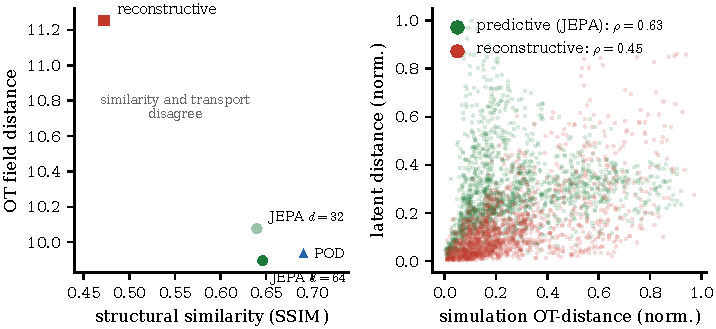
\includegraphics[width=0.9\linewidth]{sections/figures/results/fig_ot.pdf}
  \caption{Optimal-transport reconstruction comparison (Tran et al., JFM 2026)
  on test\_b. Unbalanced OT field distance by family at the impact frame, with the
  structural-similarity ranking shown alongside; the linear basis has the highest
  similarity but no transport advantage over the predictive decode, while the
  collapsed reconstructive field is correctly penalised. The Shepard panel shows
  the per-encounter alignment of latent distance with the simulation
  OT distance, predictive versus reconstructive.}
  \label{fig:ot}
\end{figure}

Finally, the wake observables tie to the structures that carry the load. A
Gaussian scale decomposition (large scale at filter width $\sigma/c = 0.05$,
following \citep{odaka2026,motoori2019}) separates the large-scale vortical
structures responsible for the lift peaks from the fine scale, applied to the
simulation field and to each family's reconstruction
(figure~\ref{fig:scale_decomp}). On test\_b the large-scale wake enstrophy of the
predictive reconstruction tracks the simulation closely (Pearson correlation
$0.89$ at impact and $0.91$ at $H = 16$, relative error $0.22$), while the
reconstructive autoencoder collapses it (correlation $0.23$ and $0.61$, relative
error near $0.8$, retaining only $16$ to $20\%$ of the large-scale amplitude and
almost none of the small-scale energy): it smooths the leading-edge vortex and
shear layer away. The linear basis has comparable large-scale correlation to the
predictive latent but worse amplitude (relative error $0.34$ to $0.38$), so the
claim is specific: the predictive latent tracks the simulation's large-scale
wake structure better than the reconstructive autoencoder on both correlation and
amplitude, and better than the linear basis on amplitude. Across the staged
encounter the simulation large-scale enstrophy rises from the gust-induced
leading-edge flux through the LEV roll-up and peak-load shedding; the predictive
reconstruction follows that rise while the reconstructive one stays flat. This is
where the wake-enstrophy advantage of \S\ref{sec:res_closure} becomes a statement
about the leading-edge vortex and shear layer rather than about a scalar.
Tracking the large-scale leading-edge vortex directly makes this quantitative.
Extracting the dominant suction-side vortex from the same $\sigma/c = 0.05$
field, the predictive decode places a coherent leading-edge vortex in all $42$
held-out encounters at $H = 16$, within $0.32$ chords of the simulation centroid
and recovering its circulation to within $5\%$, whereas the reconstructive decode
has smoothed the vortex below detection in $36$ of the $42$ (its large-scale
leading-edge amplitude falls to about a tenth of the simulation), and where it
survives its circulation error is six times larger. Per encounter the
wake-enstrophy error and the leading-edge-vortex circulation error co-vary
(Spearman $0.57$), so the scalar wake observable stands in for the position and
strength of the leading-edge vortex that produces the lift transient. The
result holds at $d = 32$; on the OOD test\_c set the predictive tracking degrades
($0.91$ to $0.65$ from impact to $H = 16$), as expected where the flow becomes
three-dimensional and the mid-plane decomposition is itself incomplete
(\S\ref{sec:flow_physics}).
\begin{figure}
  \centering
  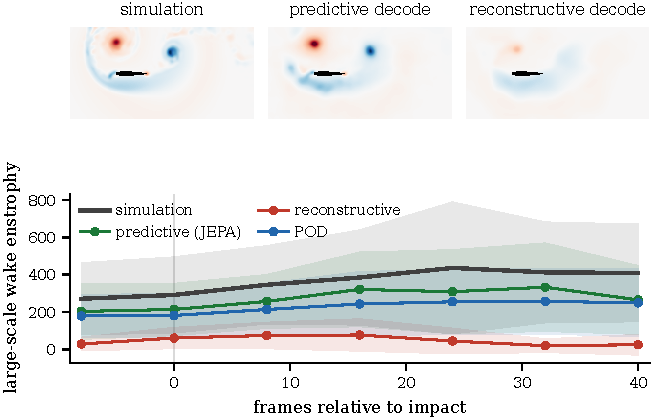
\includegraphics[width=0.98\linewidth]{sections/figures/results/fig_scale_decomp.pdf}
  \caption{Gaussian scale decomposition ($\sigma/c = 0.05$) of the held-out
  reconstructions. Top: large-scale vorticity for the simulation, the predictive
  decode, and the reconstructive autoencoder at $H = 16$; the predictive latent
  retains the leading-edge vortex and shear layer the reconstructive one smooths
  away. Bottom: large-scale wake enstrophy through the staged encounter for the
  simulation, predictive, and reconstructive fields, on each split.}
  \label{fig:scale_decomp}
\end{figure}

\subsection{Wall-pressure observability}
\label{sec:res_observability}

At deployment the vorticity field is not available; only the wall pressure is.
The representational result has an exact deployment mirror: we ask which
representation is most recoverable from a sparse set of $K$ wall-pressure taps over
a pre-impact window, using one kernel-ridge estimator across families for a uniform
comparison (the sensor placement, the lead-time prediction, and a closed-loop pilot
are detailed in Appendix~\ref{app:sensing}). Because the encoder is unconditional in
every case, this observability is unaffected by dropping the gust parameters. The
predictive state is markedly the most recoverable (figure~\ref{fig:observability}a):
with $K = 8$ taps the held-out test\_b state $R^2$ is $0.88$, against $0.58$ for the
reconstructive autoencoder and $0.32$ for the linear basis at $d = 64$, and the
contrast is sharpest at matched capacity. The energy-optimal POD coordinates,
optimal for reconstruction, are the hardest of the three to read from the wall: the
same predictive objective that produces a wake-keeping state produces one that is
also legible from pressure.

Recoverability is not estimation quality, and the distinction is itself
informative (figure~\ref{fig:observability}b). The three-dimensional
reconstructive latent is the \emph{easiest} to recover from pressure (state
$R^2 = 0.91$ at $K = 2$, the highest of any family) yet routing the impact-lift
estimate through it gives the \emph{worst} lift error (mean absolute error $1.0$
against a $C_L$ spread of $1.37$), while the predictive latent gives $0.49$; the
lift itself is read most accurately straight off the pressure ($0.39$), because
the imminent lift is already imprinted on the wall. The contribution of the
predictive latent is therefore the observable, wake-keeping state it carries, not
the instantaneous lift, which is read more accurately straight from the wall.

\begin{figure}
  \centering
  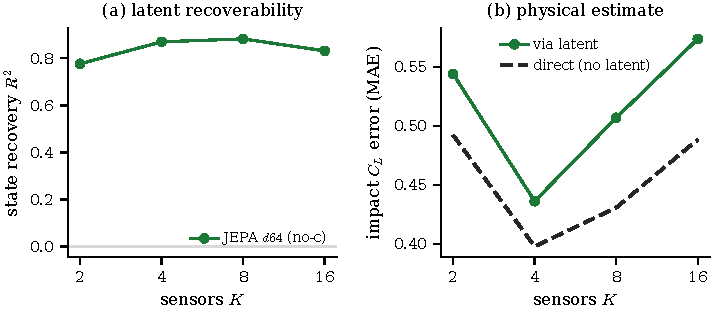
\includegraphics[width=\linewidth]{sections/figures/results/figF_observability.pdf}
  \caption{Cross-family pressure observability under the target-conditioned
  (TCSI) sensor placement. (a) Latent-state recovery $R^2$ versus sensor count
  $K$: the predictive (JEPA) state is the most recoverable at $K \ge 4$, the
  linear basis the least. (b) The physical estimate, impact $C_L$ mean absolute
  error routed through each family's recovered latent, with the direct
  pressure-to-$C_L$ baseline (dashed). The reconstructive $d = 3$ latent is the
  easiest to recover (highest $R^2$ at low $K$) yet gives the worst lift estimate,
  and the lift is read most accurately directly from the pressure.}
  \label{fig:observability}
\end{figure}
